\section{Numerical solutions in the low frequency limit}
In this section we numerically solve the linear stability problem
corresponding to Eq. \ref{iso_ode1}. We thus relax the thin-disk
assumption, using the full expressions for $\rho$, $\Omega$ and
$\kappa$, so that we may consider vertical domains up to $z\sim r$.
However, we retain the low-frequency approximation
$|\sigma^2|\ll\kappa^2$ to obtain a linear eigenvalue problem. This
level of approximation lies in between the full problem 
Eq. \ref{iso_ode}, solved by \cite{mcnally14}, and the thin-disk
limit Eq. \ref{iso_ode3}, solved by \cite{nelson13}.   

We solve Eq. \ref{iso_ode1} using a pseudo-spectral method by
expanding $W$ in Chebyshev polynomials $T_l$ up to $l=512$ and
discretizing the equation on a grid with
$\zmax=10H_\mathrm{iso}$. This procedure converts the linear problem
to a standard matrix eigenvalue problem. %In the low-frequency
%approximation the eigenvalue is $\sigma^2$. 

\subsection{Fiducial calculation}
We first validate the low-frequency approximation by solving a 
fiducial problem with $q=-1$, $p=-1.5$, $\epsilon=0.1$ and $k_x =
200\pi/r$ with solid boundaries. This is the setup considered by
\cite{mcnally14} who solved the full problem. 

Fig. \ref{lowfreq_eigen} shows the eigenvalues $\sigma = \omega +
\ii\nu$. This plot is effectively identical to that in
\cite{mcnally14}. The low-frequency approximation reproduces the
three solution branches defined by \citep{nelson13}: corrugation modes
with odd symmetry, breathing modes with even symmetry, and surface
modes which correspond to the nearly-vertical locus in
Fig. \ref{lowfreq_eigen}. 

\begin{figure}
  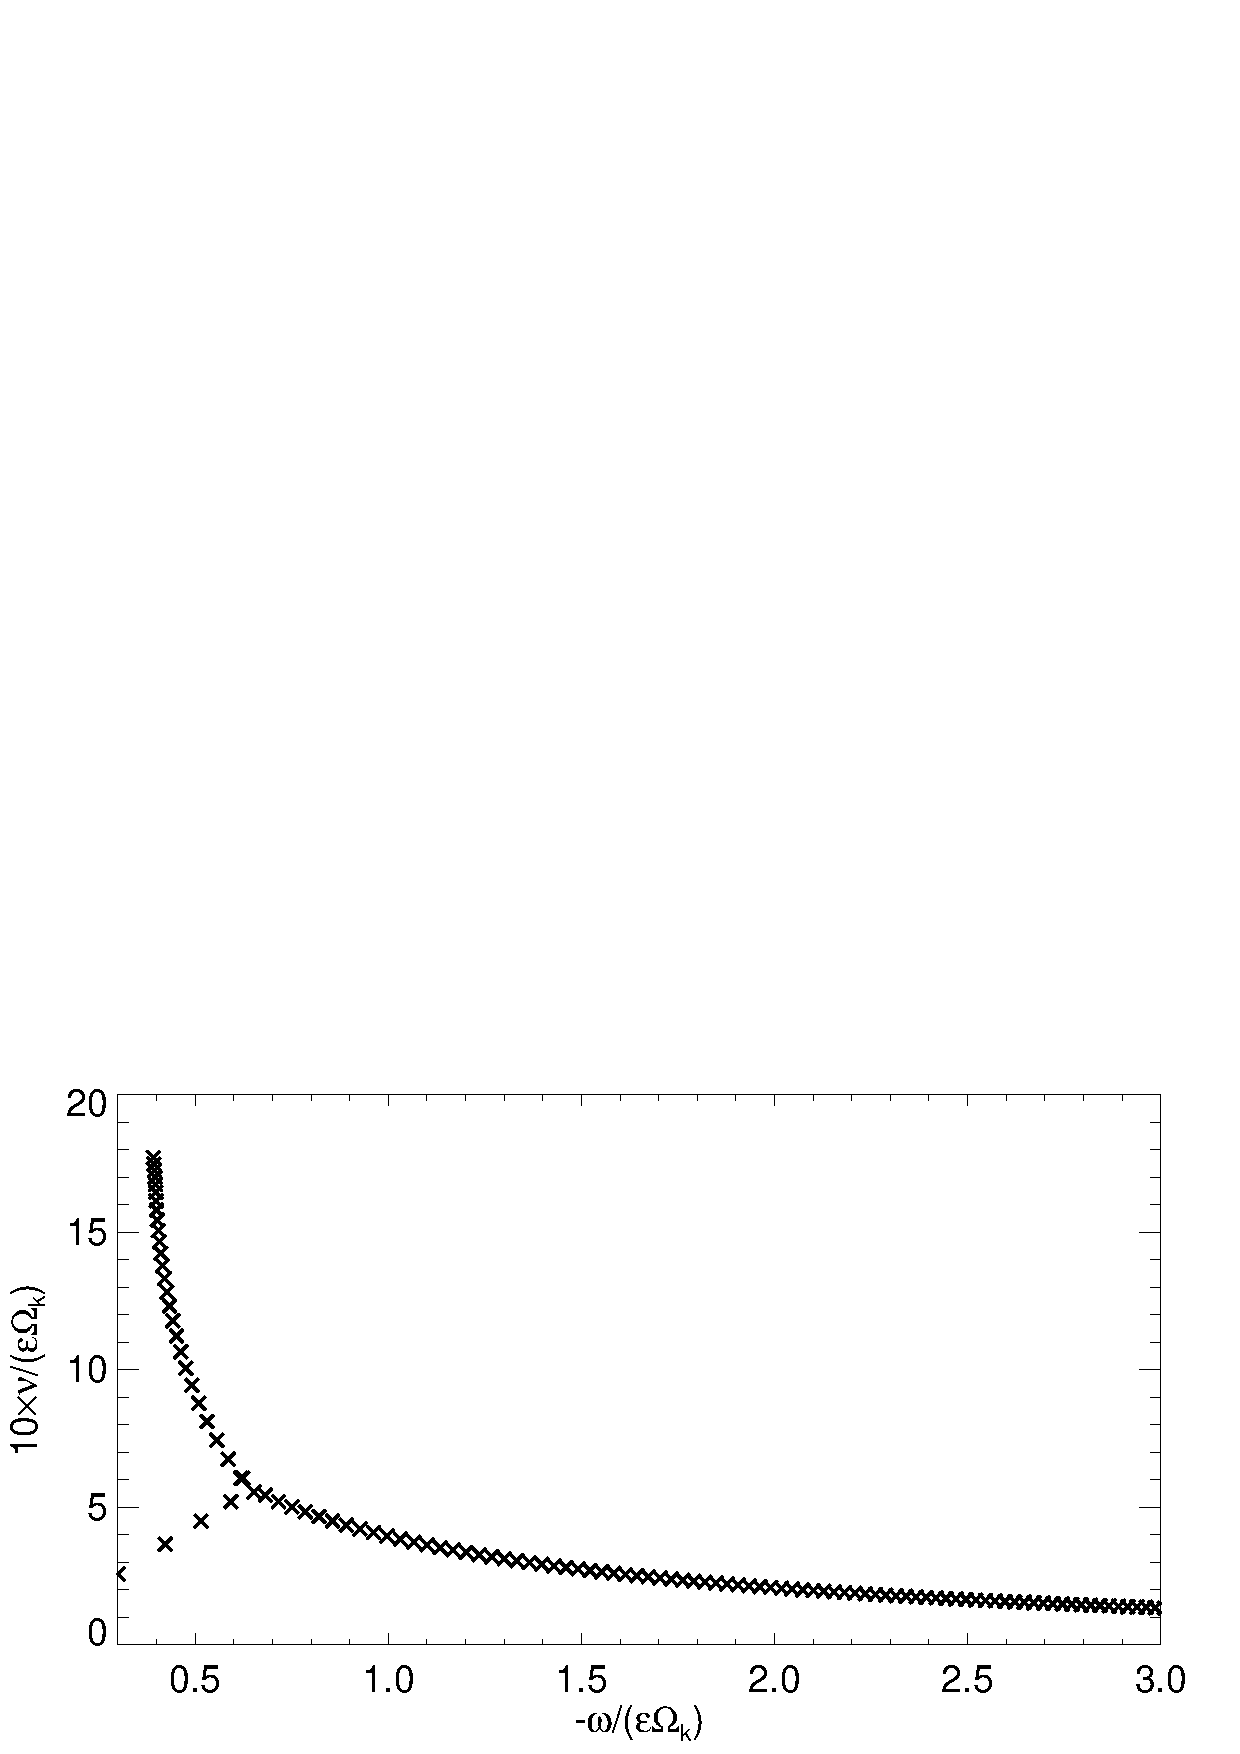
\includegraphics[width=\linewidth]{figures/eigenvalues_iso}
  \caption{Eigenvalues in the low-frequency approximation for the
    vertical shear instability in a vertically isothermal disk evolved
    isothermally ($\gamma=\Gamma=1$). The disk parameters are $q=-1$,
    $p=-1.5$ and $\epsilon=0.1$, while the perturbation radial
    wavenumber is $k_x=200\pi/r$. This is the set up considered in
    \cite{mcnally14}. \label{lowfreq_eigen}
  }
\end{figure}

We plot in Fig. \ref{lowfreq_eigenfunc} the structurally simplest
eigenfunction --- the fundamental corrugation mode corresponding to
the eigenvalue with $\mathrm{min}|\sigma|$. The perturbation $W$ is
roughly proportional to $z$, except close the boundaries where it
flattens because $\delta v_z=dW/dz=0$ is imposed there. 

For $k_x = 200\pi/r$ and $\epsilon = 0.1$, the dimensionless
wavenumber $\hat{k} = k_xH_\mathrm{iso}=20\pi$. Then the expected
growth rate according to Eq. \ref{simple_growth} with $M=1$ is
\begin{align*}
  \nu = 0.2606\epsilon\Omega_k,
\end{align*}
as obtained numerically (Fig. \ref{lowfreq_eigen}). This agreement is
surpsingly good, given that Eq. \ref{simple_growth} assumes the
thin-disk approximation and imposes a different boundary condition to
that in the numerical calculations. 

\begin{figure}
  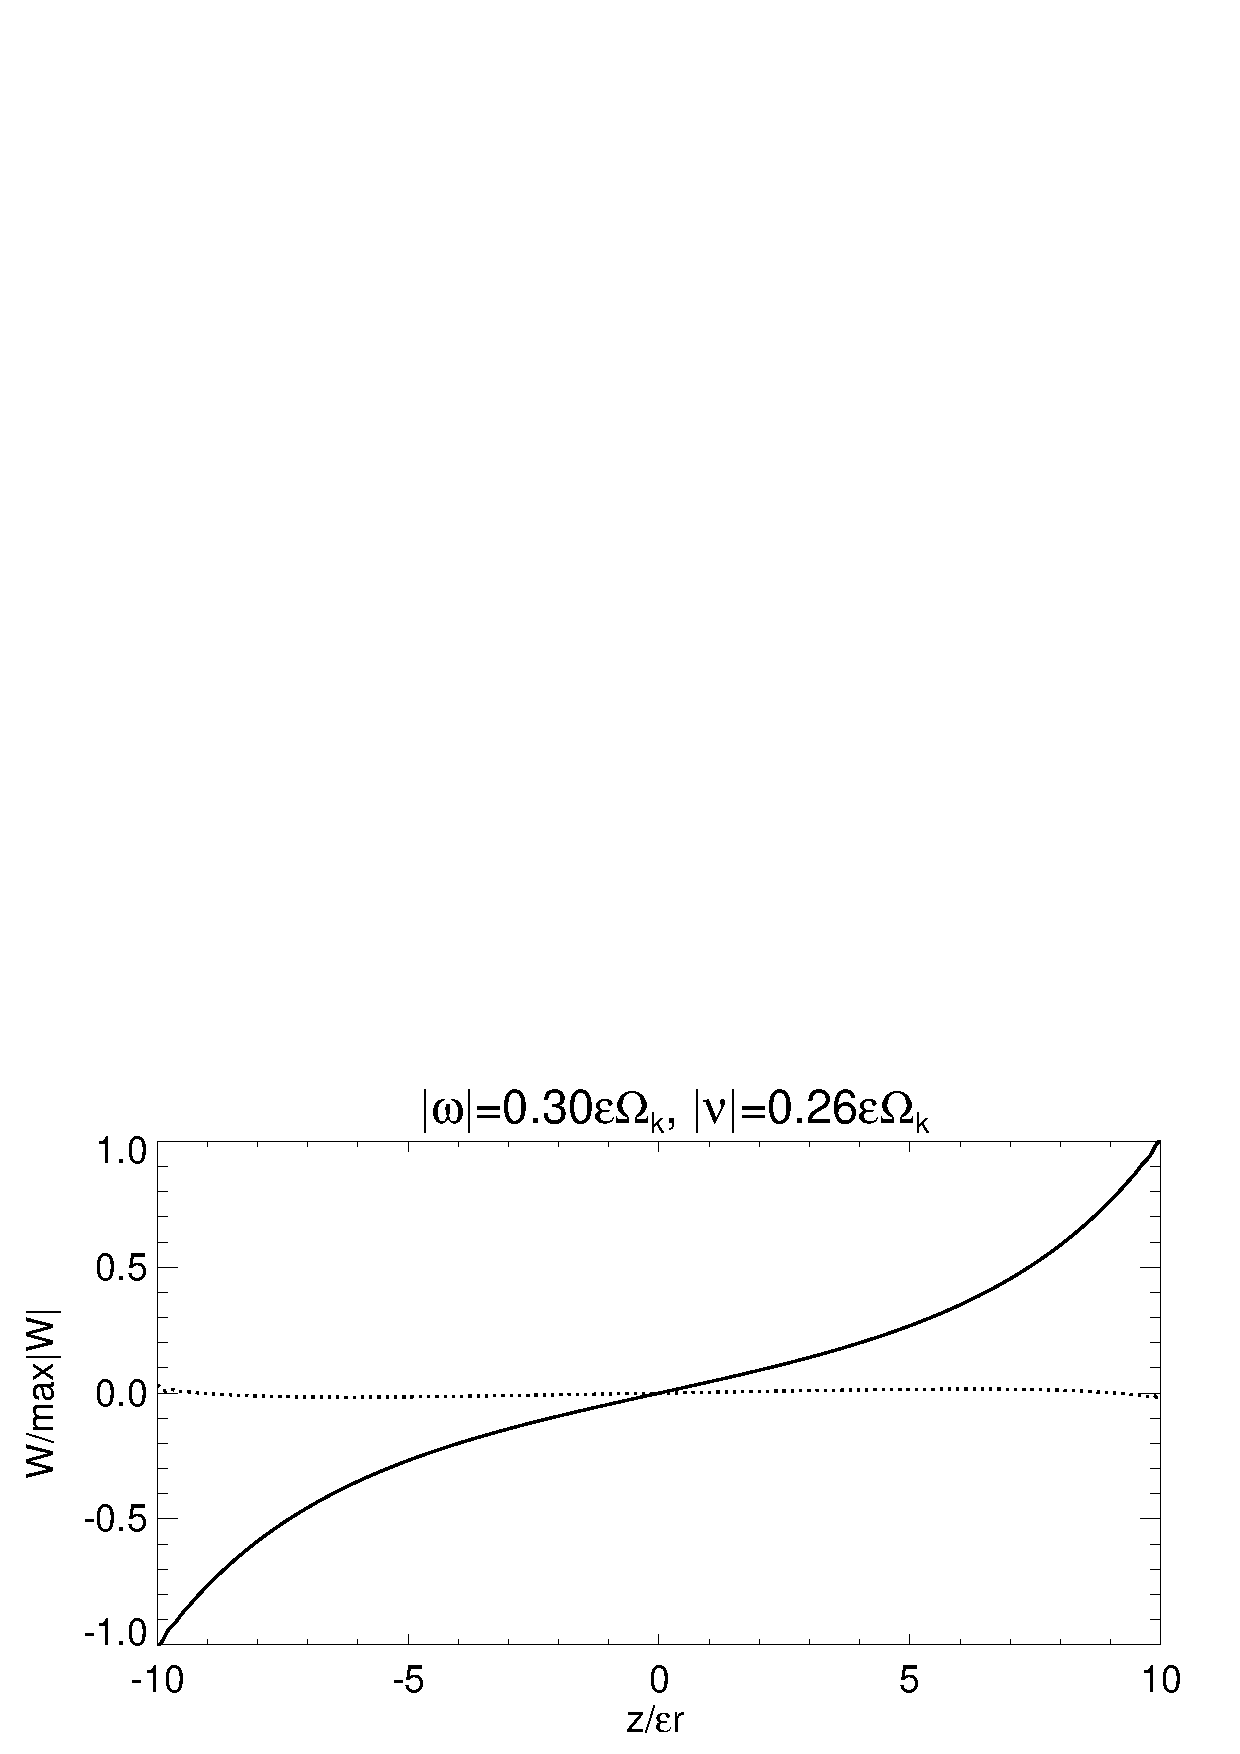
\includegraphics[width=\linewidth]{figures/eigenvector_iso}
  \caption{Eigenfunction of the fundamental corrugation mode,
    corresponding to the 
    bottom-left eigenvalue displayed in Fig. \ref{lowfreq_eigen}. The
    solid and dashed lines are $\real W$ and $\imag W$, respectively. 
    \label{lowfreq_eigenfunc}
  }
\end{figure}
